% ALGUNOS PAQUETES REQUERIDOS (EN UBUNTU): %
% ========================================
% %
% texlive-latex-base %
% texlive-latex-recommended %
% texlive-fonts-recommended %
% texlive-latex-extra %
% texlive-science %
% texlive-lang-spanish (en ubuntu 13.10) %
% ******************************************************** %

\documentclass[a4paper]{article}
\usepackage[spanish, es-nodecimaldot, es-noquoting]{babel}
\usepackage[utf8]{inputenc}
\usepackage{fancyhdr}
\usepackage[pdftex]{graphicx}
\usepackage{sidecap}
\usepackage{caption}
\usepackage{subcaption}
\usepackage{booktabs}
\usepackage{makeidx}
\usepackage{float}
\usepackage{amsmath, amsthm, amssymb}
\usepackage{amsfonts}
\usepackage{sectsty}
\usepackage{wrapfig}
\usepackage{listings}
\usepackage{pgfplots}
\usepackage{pgfplotstable}
\usepackage{enumitem}
\usepackage[hidelinks]{hyperref}
\usepackage{listings}
\usepackage{listingsutf8}
\usepackage{tkz-graph}
\usepackage{multirow}
\usepackage{tikz}
\usetikzlibrary{arrows.meta}

\linespread{factor}

\definecolor{mygreen}{rgb}{0,0.6,0}
\definecolor{mygray}{rgb}{0.5,0.5,0.5}
\pgfplotsset{compat=1.8}
\setlist[enumerate]{label*=\arabic*.}
\lstset{
	inputencoding=utf8/latin1,
	language=C++,
	basicstyle=\ttfamily,
	keywordstyle=\bfseries\color{blue},
	stringstyle=\color{red}\ttfamily,
	commentstyle=\color{mygreen}\ttfamily,
	morecomment=[l][\color{magenta}]{\#},
	numbers=left,
	numberstyle=\color{mygray}
}

\usepackage{fancyhdr}
\pagestyle{fancy}
\fancyhf{}
\fancyhead[LO]{Problemas, Algoritmos y Programación}
\fancyhead[RO]{Trabajo Práctico N\textsuperscript{o} 1}
%\fancyfoot[LO]{\small{Shai Bianchi, Martín Jedwabny, Manuel Mena, Iván Pondal}}
\fancyfoot[RO]{\thepage}
\renewcommand{\headrulewidth}{0.5pt}
\renewcommand{\footrulewidth}{0.5pt}
\setlength{\textwidth}{16cm}
\setlength{\hoffset}{-1.1cm}
\setlength{\headsep}{0.5cm}
\setlength{\textheight}{25cm}
\setlength{\voffset}{-1.75cm}
\setlength{\headwidth}{\textwidth}
\setlength{\headheight}{13.1pt}
\renewcommand{\baselinestretch}{1.1} % line spacing

\usepackage{caratula}

\allowdisplaybreaks
\newcommand{\ord}{\ensuremath{\operatorname{O}}}
\newcommand{\nat}{\ensuremath{\mathbb{N}}}
\newcommand{\acr}[1]{\lowercase{\textsc{#1}}}
\newcommand{\comp}{\ensuremath{^{\operatorname{C}}}}
\newcommand{\argmax}{\operatornamewithlimits{arg\,m\acute{a}x}}

\newcommand{\subheading}[1]{\vspace{1em} \noindent\textbf{#1} \nopagebreak
\smallskip \nopagebreak}

% Lemas, definiciones, etc.
\theoremstyle{plain}
  \newtheorem{theorem}{Teorema}
  \newtheorem{prop}{Proposición}
  \newtheorem{lema}{Lema}
\theoremstyle{remark}
  \newtheorem{obs}{Observación}
\theoremstyle{definition}
  \newtheorem{defi}{Definición}

% Pseudocódigo
\usepackage[onelanguage, spanish]{algorithm2e}
    % \NoCaptionOfAlgo
    \LinesNumbered\RestyleAlgo{ruled}\IncMargin{1em}\DontPrintSemicolon
    \SetArgSty{}\SetCommentSty{textsf}\SetFuncSty{textsf}
    \SetKwInput{Input}{Entrada}
    \SetKwInput{Output}{Salida}
    \SetKwProg{For}{para}{ hacer}{fin}
    \SetKwProg{Fn}{función}{:}{fin}

\begin{document}
\materia{Problemas, Algoritmos y Programación}
\submateria{Segundo cuatrimestre de 2016}
\titulo{Trabajo Práctico N\textsuperscript{o} 2}
\integrante{Ken Thompson}{867/5309}{ken\_thompson\_k-po@jennymail.com}
% \integrante{Shai Bianchi}{540/12}{bianchishai@gmail.com}
% \integrante{Martín Jedwabny}{885/13}{martiniedva@gmail.com}
% \integrante{Manuel Mena}{313/14}{manuelmena1993@gmail.com}
% \integrante{Iván Pondal}{078/14}{ivan.pondal@gmail.com}

\maketitle
% no footer on the first page

% group hash
% seed = 2^32 + 42
% \vspace*{\fill}
% \begin{center}
% 8796613900571664
% \end{center}
% \vspace*{\fill}

% \thispagestyle{empty}

\newpage
\tableofcontents

\newpage
\section{Ejercicio 1}

Peso asignado: 9.

\subsection{Introducción}

Se tiene un mapa de $N$ esquinas y $M$ calles bidireccionales en donde las
esquinas pueden ser casas de alumnos de secundaria, escuelas o esquinas
neutrales. El problema consiste en encontrar la mínima cantidad de esquinas en
las que podemos podemos poner a un estudiante del departamento a contar sobre
la carrera de Ciencias de la Computación, de modo tal que no importe qué
camino utilice cada chico para llegar de su casa al colegio, ni a qué colegio
vaya cada chico, siempre tenga que pasar por una esquina donde lo podamos
interceptar para contarle de la carrera.

\subsection{Solución propuesta}

La resolución de este ejercicio consiste en modelar el mapa como un grafo, y
más específicamente como una red de flujo, y obtener el flujo máximo. En esta
red de flujo se tiene las casas de los estudiantes conectadas a la fuente y
las escuelas al sumidero (pero podría ser al revés y no afectaría en lo
absoluto).

Las capacidades de las aristas serán de 1, pero además también deben tener
capacidad 1 los nodos. Para modelar las capacidades de los vértices, se
representó cada uno de ellos como un arco de capacidad 1 cuyos extremos son un
nodo en donde inciden todas las aristas que incidirían en el vértice original
y otro con todas las aristan salientes.

\begin{figure}[H]
\centering
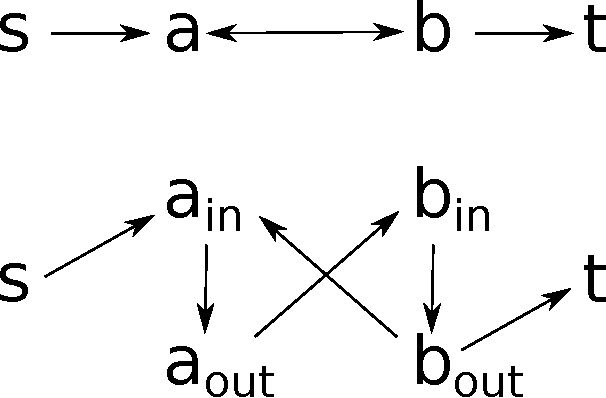
\includegraphics[scale=0.6]{imagenes/ej1_capacidades_nodos.pdf}
\end{figure}

Se construye la red residual y luego se aplica el ya conocido algoritmo de
\textit{Edmonds-Karps} para conocer el flujo máximo.

\subsubsection*{Detalles implementativos}

La estructura utilizada para la representación de la red fue un vector de
listas de enteros (lista de adyacencias). Se reservaron las dos primeras
posiciones del vector para la fuente(0) y el sumidero(1).

El modelado de vértices con capacidades através de aristas con un nodo para
las entradas y otro para las salidas se realiza en el momento mismo de la
lectura de la entrada. El vector de listas contiene exactamente $2N + 2$
elementos, siendo $N$ la cantidad de esquinas. Esto se debe a que por cada
esquina existirán dos nodos(el de entrada y el de salida) y se tiene dos
espacios mas para la fuente y el sumidero.

Al realizar la lectura se tienen dos ciclos. El primero lee el tipo de cada
esquina. Si es una casa de alumno entonces se agrega el nodo de entrada a los
vecinos de la fuente. Si es escuela se agrega el sumidero a los vecinos de el
nodo de salida. Y si es una esquina neutral no se tiene un trato especial.
Para los tres casos se agrega el nodo de salida como único incidido por el
nodo de entrada.

El segundo ciclo simplemente realiza la lectura de ejes, agregando el nodo de
entrada de uno como incidido por el nodo de salida del otro y viceversa.

Una vez hecho esto ya se tiene una red lista para ser procesada.

\subsubsection*{Pseudocódigo}


\begin{algorithm}[]
	\caption{flujoMáximo}
	\Input{$Vector<Lista<Entero>>$ $redResidual$}
	\Output{$Entero$ $flujoMaximo$}

	$flujo$ $\gets$ 0 \;
	$Lista<Entero>$ $camino$ $\gets$ BFS($redResidual$, FUENTE, SUMIDERO) \;
	\While{$\neg camino$.vacio()} {
		recorrerCaminoDeAumento($redResidual$, $camino$) \;
		$camino$ $\gets$ BFS($redResidual$, FUENTE, SUMIDERO) \;
		$flujo$ $\gets$ $flujo + 1$ \;
	}
	\Return $flujo$ \;
\end{algorithm}

\begin{algorithm}[]
	\caption{recorrerCaminoDeAumento}
	\Input{$Vector<Lista<Entero>>$ $redResidual$(por referencia), $Lista<Entero>$ $camino$}

	$Iterador<Lista<Entero>>$ $itCamino$ $\gets$ $camino$.Primero() \;
	\While{$itCamino$.siguiente() $\not=$ $camino$.Fin()} {
		Entero $desde$ $\gets$ *$itCamino$ \;
		Entero $hasta$ $\gets$ *($itCamino$.siguiente()) \;
		$redResidual$[$desde$].borrar($hasta$) \;
		$redResidual$[$hasta$].agregar($desde$) \;
		$itCamino$++ \;
	}
\end{algorithm}

Notar que en recorrerCaminoDeAumento se borran y agregan aristas porque las
capacidades de las mismas son siempre 1. De lo contrario habría que tenerse en
cuenta la capacidad de las mismas, no se borrarían y agregarían sino que se
aumentaría o restaría el flujo que pasa por el eje.

\subsection{Correctitud}

Lo que el algoritmo debe devolver es la minima cantidad de esquinas a donde
puedan situarse estudiantes de modo tal que cada alumno de secundaria siempre
tenga que pasar por una de estas esquinas sin importar que camino tome o a que
colegio vaya.

En otras palabras, existen conjuntos de esquinas para los cuales todos los
caminos de las casas a las escuelas pasan por al menos una de las esquinas del
conjunto. El que interesa es el de mínimo cardinal (un conjunto que tenga
todas las esquinas por supuesto que cumpliría el requisito de interceptar los
alumnos, pero no sería mínimo).

Este conjunto de mínimo cardinal representa un cuello de botella en cuanto a
los caminos que los alumnos de secundaria pueden elegir.

Lo que el algoritmo devuelve es el valor flujo máximo. Por teorema se sabe que
el valor del flujo máximo es igual a la capacidad del corte mínimo.

Lo que hace que la capacidad del corte mínimo en esta red de flujo represente
el cardinal del conjunto de esquinas es el hecho de que los vértices tengan
capacidad 1. Esto provoca que la capacidad del corte no este dada por la
capacidad de las aristas salientes sino por la cantidad de nodos del corte que
tienen aristas salientes. Entonces si para cualquier corte de esta red de
flujo, su capacidad es igual a la cantidad de nodos con aristas salientes, es
decir, esquinas de las cuales salen caminos, consiguiendo el corte mínimo se
obtendría el cuello de botella y su capacidad sería el cardinal del conjunto.

Entonces el valor del flujo máximo de esta red es la mínima cantidad de
esquinas en las que deben situarse estudiantes para poder interceptar a todos
los alumnos sin importar qué caminos tomen o a qué escuela asistan.

\subsection{Complejidad}

Lo primero a analizar es la lectura de la entrada. Previamente se detalló el
procedimiento que constaba de dos ciclos. El primero lee las $N$ esquinas y al
hacerlo las agrega a la correspondiente lista en tiempo constante, por lo que
ese ciclo tiene complejidad temporal $\ord(N)$. El segundo lee las $M$ calles
y también realiza la correspondiente inclusión en una lista en tiempo
constante, por lo que la complejidad es $\ord(M)$. La complejidad temporal de
la lectura es $\ord(M + N)$.

Hecho esto la cantidad de nodos de la red de flujo es de $2N + 2$ debido a que
cada nodo es representado por una arista como fue especificado anteriormente,
lo cual inserta dos nodos por esquina, y a que se tiene dos nodos adicionales
que representan la fuente y el sumidero. La cantidad de aristas es $2M + N$
porque por cada calle se agregan 2 aristas ya que son bidireccionales, y cada
esquina también es una arista.

Si a este grafo se le aplica el algoritmo de \textit{Edmonds-Karps}, que es
$\ord(E^2V)$, la complejidad queda $\ord((2M + N)^2(2N + 2))$.

Como el grafo es conexo ya que existe un camino entre cada par de esquinas se
sabe que $N \leq M + 1$ por lo que podemos acotarlo quedando de esta forma la
complejidad $\ord((2M + M + 1)^2(2N + 2)) = \ord(M^2N)$.

\subsection{Casos de prueba}

Para evaluar el código desarrollado además de ver que diera los resultados
correctos en las entradas provistas por el enunciado se realizaron las
siguientes pruebas:

\begin{itemize}
	\item Camino simple
	\item Grafo moño: este grafo es el que tiene muchas casas, muchas
	escuelas, y todas pasan por una única esquina neutral, siendo esta el
	cuello de botella.
	\item Caminos atravesados: este grafo es el representado en la figura
	\ref{ej1:atravesados}. El propósito de esta prueba es chequear el correcto
	funcionamiento de la red residual y los caminos de aumento. Debido a la
	topología del grafo es posible que el \textit{BFS} devuelva el camino en
	zigzag. Al tocar los nodos que el siguente camino contemplará debe tenerse
	cuidado de no haber manipulado de forma errónea los el camino de aumento
	de manera tal que el segundo camino encontrado no este cortado.
	\item Una casa y una escuela: estos dos casos cumplen el propósito de
	corroborar que las escuelas y casas hayan sido teniadas en cuenta como
	posibles cuellos de botella, no solamente las esquinas neutrales.
	\item Casos normales grandes donde se prueba el algoritmo en general.
\end{itemize}

\begin{figure}[H]
	\caption{Caminos atravesados}
	\label{ej1:atravesados}
	\centering
	\begin{tikzpicture}[x=1.5cm ,y=1.5cm]
		\SetGraphUnit{2}
		\GraphInit[vstyle=Normal]
		\Vertex[L=$A_1$]{A1}
		\EA[L=$A_2$](A1){A2}
		\SO[L=$X_1$](A1){X1}
		\SO[L=$X_2$](A2){X2}
		\SO[L=$X_3$](X1){X3}
		\SO[L=$E_1$](X3){E1}
		\SO[L=$E_2$](X2){E2}
		\Edge(A2)(X2)
		\Edge(X3)(X1)
		\Edge(X3)(E1)
		\SetUpEdge[style={ultra thick}, color=red]
		\Edge(A1)(X1)
		\Edge(X2)(X1)
		\Edge(X2)(E2)
	\end{tikzpicture}
\end{figure}

\newpage
\section{Ejercicio 2}

\newpage
\section{Ejercicio 3}

Peso asignado: 9.

\subsection{Problema}

El enunciado pide, dadas N esquinas y M calles bidireccionales resolver Q queries de varios tipos:
\begin{itemize}
	\item[A: ] dadas dos esquinas e1 y e2, imprimir la cantidad de calles que en caso de ser cortadas impiden llegar de e1 a e2.
	\item[B: ] dada una calle, imprimir un 1 si al cortar la calle existen al menos dos esquinas entre las que deja de haber un camino, y 0 en caso contrario.
	\item[C: ] dada una esquina e1, imprimir la cantidad de esquinas e2 tales que de cortar una sola calle, sea cual sea, seguir\'a habiendo camino de e1 a e2.
\end{itemize}

El modelo que se plantea entonces es representar las esquinas y calles como nodos y aristas respectivamente, de un grafo no dirigido
(porque las calles son bidireccionales).\\

Se asegura que el grafo es conexo (pues hay un camino para cada par de esquinas) y que hay una cantidad positiva de nodos y aristas.
Además, no hay calles que conectan las mismas esquinas, por lo cual no habrá ejes repetidos. \\

Debido a la complejidad que se pide y que el grafo es conexo (hay al menos tantos aristas como vértices menos uno) y el algoritmo y nociones
vistas en clase para calcular Componentes Biconexas Maximales se va a querer representar los aristas del grafo como listas de adyacencia para as\'i 
recorrer los nodos del grafo en tiempo lineal con respecto a la cantidad de aristas mediante DFS. Luego mas adelante se ve que las queries se resuelven
calculando puentes y otras propiedades entre los nodos del grafo mediante DFS. \\

Finalmente se debe imprimir el resultado de cada query seg\'un su tipo, lo cual se explica en detalle en la sección de Correctitud. \\

\subsection{Algoritmo e intuición}

\subsubsection*{Pseudocódigo}

Sea la clase $Grafo = <Vertices, Aristas, ListaAdyacencia>$
	donde Vertices y Aristas son Enteros que representan la cantidad de vértices y aristas del grafo y
	ListaAdyacencia es un $Vector<Lista<Par<Entero, Entero>>>$ donde
	el tamaño del vector es Vertices y por cada arista que conecta nodos v 
	y w del grafo representado, ListaAdyacencia[v] incluye $<e, w>$ y
	ListaAdyacencia[w] incluye $<e, v>$ donde $e$ es el número de arista (entre 0 y Aristas-1).

\begin{algorithm}[]
    \caption{ResolverQueries}
    \Input{Grafo $grafo$, Queries $queries$}
    $Vector<Bool>$ $puentes \gets [false,...,false]$ con size grafo.Aristas \;
	$Vector<Entero>$ $depth \gets [-1,...,-1]$ con size grafo.Vertices \;
	$Vector<Entero>$ $low \gets [-1,...,-1]$ con size grafo.Vertices \;
	\emph{CalcularPuentesDFS$(grafo, puentes, depth, low, 0, 0, 0)$} \;
	$Vector<Entero>$ $componente\_puente\_del\_vertice \gets [-1,...,-1]$ con size grafo.Vertices \;
	$Vector<Entero>$ $vertices\_del\_componente\_puente \gets [0,...,0]$ con size grafo.Vertices \;
	$Variable$ $Global$ $Entero$ $contador\_componentes \gets 0$ \;
	\emph{CalcularComponentesPuenteDFS$(grafo, puentes, componente\_puente\_del\_vertice, $ $ vertices\_del\_componente\_puente, 0, contador\_componentes, 0)$} \;
	\For{$query$ en $queries$} {
		\If{$query.tipo$ == A} {
			$Vector<Bool>$ $visitado \gets [false,...,false]$ con size grafo.Vertices \;
			\emph{Imprimir PuentesEntreNodos$(grafo, puentes, visitado, query.esquina1, query.esquina2, query.esquina1)$}
		}
		\If{$query.tipo$ == B} {
			\emph{Imprimir $puentes[query.calle]$}
		}
		\If{$query.tipo$ == C} {
			$Entero$ $n$ \;
			$n \gets vertices\_del\_componente\_puente[componente\_puente\_del\_vertice[query.esquina]]$ \;
			\emph{Imprimir n-1}
		}
	}
\end{algorithm}

\begin{algorithm}[]
    \caption{CalcularPuentesDFS}
    \Input{Grafo $grafo$, Vector$<Bool>$ $puentes$, Vector$<Entero>$ $depth$, Vector$<Entero>$ $low$, Entero $v$, Entero $d$, Entero $padre$}
    $depth[v] \gets d$ \;
	$low[v] \gets d$ \;
	\For {$<e, w>$ en $grafo.ListaAdyacencia[v]$ tal que $w$ != $padre$} {
		\eIf{$depth[w]$ == -1}{
			\emph{CalcularPuentesDFS$(grafo, puentes, depth, low, w, d+1, v)$} \;
			$low[v] \gets min(low[v], low[w])$ \;
			\If {$low[w] >= depth[w]$} {
				$puentes[e] \gets true$
			}
		}{
			$low[v] \gets min(low[v], depth[w])$ \;
		}
	}
\end{algorithm}

\begin{algorithm}[]
    \caption{CalcularComponentesPuenteDFS}
    \Input{Grafo $grafo$, Vector$<Bool>$ $puentes$, Vector$<Entero> componente\_puente\_del\_vertice$, Vector$<Entero> vertices\_del\_componente\_puente$, Entero $v$, Variable Global Entero $contador\_componentes$, Entero $componente\_actual$}
    $componente\_puente\_del\_vertice[v] \gets componente\_actual$ \;
    $vertices\_del\_componente\_puente[componente\_actual]++$ \;
    \For {$<e, w>$ en $grafo.ListaAdyacencia[v]$} {
    	\If {$componente\_puente\_del\_vertice[w]$ == -1} {
			\eIf {$puentes[e]$} {
				$contador\_componentes++$ \;
				$Entero$ $componente \gets contador\_componentes$ \;
				\emph{CalcularComponentesPuenteDFS($grafo, puentes, componente\_puente\_del\_vertice,$ 
				$vertices\_del\_componente\_puente, w, contador\_componentes, componente$)} \;
			}{
				\emph{CalcularComponentesPuenteDFS($grafo, puentes, componente\_puente\_del\_vertice,$ 
				$vertices\_del\_componente\_puente, w, contador\_componentes, componente\_actual$)}
			}
		}
    }
\end{algorithm}

\begin{algorithm}[H]
    \caption{PuentesEntreNodos}
    \Input{Grafo $grafo$, Vector$<Bool>$ $puentes$, Vector$<Bool>$ $visitado$, Entero $src$, Entero $dst$, Entero $actual$}
    $visitado[actual] \gets true$ \;
    \If {$actual == dst$} {
    	\Return{0}
    }
    $Entero$ $ans \gets -1$ \;
    \For {$<e, w>$ en $grafo.ListaAdyacencia[v]$} {
    	\If {$visitado[w]$ == $false$} {
			$Entero$ $rec \gets$ PuentesEntreNodos$(grafo, puentes, visitado, src, dst, w)$ \;
			\If{$rec$ != -1} {
				$ans \gets puentes[e]$ ? $rec+1$ : $rec$
			}
		}
    }
    \Return{ans}
\end{algorithm}

\subsubsection*{Estrategia}

Primero se calculan los ejes puentes con un algoritmo similar al que calcula Componentes Biconexas Maximales. Por esto
se guardan los ejes del grafo como lista de adyacencia y para cada eje se guarda su numero de eje (as\'i despu\'es los podemos
marcar rápido como eje puente). Se recorre el grafo mediante DFS y as\'i podemos garantizar que su complejidad sera lineal 
con respecto a la cantidad de vertices y aristas. \\
Luego se separan los nodos en Bridge Components (explicación en la secci\'on siguiente). Esto lo hacemos tambi\'en mediante DFS. \\
Finalmente se contesta cada query seg\'un los datos calculados previamente excepto en el caso de las queries tipo A en cuyo caso 
se calculan los aristas puentes entre los nodos que representan las esquinas. Nuevamente se usa DFS. \\
A lo largo de todos los algoritmos se va manteniendo vectores de longitud grafo.Aristas o grafo.Vertices para ir guardando resultados
parciales y nodos visitados en cada recorrido DFS del grafo. \\

\subsection{Correctitud}

\subsubsection*{ResolverQueries}
Esta es la función principal del algoritmo. Dado el grafo y las queries de entrada se crea un vector $puentes$ 
que contiene para cada arista si es puente o no, lo cual se quiere calcular a continuaci\'on. \\
Es importante notar que por la forma en que se crea la clase Grafo y se rellena, cada eje tiene un número 
único entre 0 y la cantidad de aristas menos uno. \\
Luego se crean dos vectores $depth$ y $low$ de tamaño cantidad de vértices del grafo. Con esto se calculan los
ejes puente mediante la funci\'on CalcularPuentesDFS. El nodo inicial de CalcularPuentesDFS es arbitrario 
mientras sea el mismo que el padre inicial, por lo cual se define al nodo 0 como el inicial. Además queremos 
que el $depth$ inicial sea 0 ya que es la profundidad inicial de los nodos según el algoritmo para calcular 
Componentes Biconexas Maximales explicado en clase, que es en definitiva el esquema que sigue la funcio\'n 
CalcularPuentesDFS. \\
Habiendo calculado los aristas puente, ahora se quiere calcular para cada nodo e1, la cantidad de nodos e2 
tales que de cortar una sola arista, sea cual sea, seguir\'a habiendo un camino de e1 a e2. \\
Como el grafo es conexo, las nodos inicialmente están conectados. Dada el nodo e1, si existe una arista tal que al 
cortarla e1 y otro nodo se desconectan entonces seguro que esa arista es un puente (por la definición de puente). 
De hecho, si corto una arista que no es puente, el grafo sigue siendo conexo. \\
El problema es cuando e1 y e2 forman un puente o pertenecen a diferentes componentes biconexas maximales, es decir, 
cuando hay un puente entre ellos. Debido a eso, e1 y e2 siguen estando conectados no importa cual arista sea cortada
si y solo si pertenecen a una misma componente biconexa maximal que no sea un puente. \\
Entonces es posible seguir llegando de un nodo e1 a otro e2 habiendo cortado una calle 
cualquiera, mientras no hayan aristas puente entre ellos. Si hay un arista puente entre ellos, cortarlo basta para desconectarlos. \\
Con esta motivación definimos los Bridge Components del grafo. Estos componentes se obtienen condensando cada componente biconexa 
maximal que no es un puente en un solo nodo. \\

Ejemplo:\\

\begin{figure}[H]
\caption{Grafo original}
\centering
\begin{tikzpicture}
\begin{scope}[every node/.style={circle,thick,draw}]
    \node (A) at (0,0) {A};
    \node (B) at (0,2) {B};
    \node (C) at (1,1) {C};
    \node (D) at (3,1) {D};
    \node (E) at (4,0) {E};
    \node (F) at (4,2) {F};
\end{scope}

\begin{scope}[>={Stealth[black]},
              every node/.style={fill=white,circle},
              every edge/.style={draw=black,very thick}]
    \path [-] (A) edge (B);
    \path [-] (A) edge (C);
    \path [-] (B) edge (C);
    \path [-] (C) edge[draw=red] (D);
    \path [-] (D) edge (E);
    \path [-] (E) edge (F);
    \path [-] (F) edge (D); 
\end{scope}
\end{tikzpicture}
\end{figure}

\begin{figure}[H]
\caption{Grafo condensado en Bridge Components}
\centering
\begin{tikzpicture}
\begin{scope}[every node/.style={circle,thick,draw}]
    \node (A) at (0,0) {A,B,C};
    \node (D) at (2,0) {D,E,F};
\end{scope}

\begin{scope}[>={Stealth[black]},
              every node/.style={fill=white,circle},
              every edge/.style={draw=black,very thick}]
    \path [-] (A) edge[draw=red] (D);
\end{scope}
\end{tikzpicture}
\end{figure}

El algoritmo CalcularComponentesPuenteDFS hace esto guardando para cada nodo 
a qué Bridge Component pertenece en el vector $componente\_puente\_del\_vertice$ y para cada uno de esos componentes, 
$vertices\_del\_componente\_puente$ guarda cuántos nodos tiene ese componente. \\
Ahora bien, los nodos dentro de cada Bridge Component están conectados de manera tal que no hay puentes entre ellos,
por lo cual si corto cualquier arista del grafo siguen estando conectados entre si.

Finalmente, el algoritmo resuelve las queries según su tipo correspondiente:
\begin{itemize}
	\item[A: ] dado que se quiere imprimir la cantidad de calles que, en caso de ser cortadas impiden llegar de la 
	esquina e1 a e2, cuenta mediante la función PuentesEntreNodos y el vector $puentes$, los puentes entre los nodos 
	del grafo que representan esas esquinas.
	\item[B: ] se fija en el vector $puentes$ si la calle es un puente o no y lo imprime.
	\item[C: ] dada una esquina e1 se quiere imprimir la cantidad de esquinas e2 tales que de cortar una calle cualquiera 
	sigue habiendo camino de e1 a e2. Como se explico, esto es exactamente la cantidad de nodos en el Bridge Component del
	grafo, que son justamente los nodos e2 que están conectados a e1 sin puentes entre e1 y e2, entonces sin importar
	qué calle se corte, seguirán estando conectados. Los demás nodos son posibles de desconectar de e1 cortando alguno
	de los aristas puentes entre e1 y esos nodos. Notar que a esta cantidad se le resta 1 para no contar a e1 en su 
	propio Bridge Component.
\end{itemize}

\subsubsection*{CalcularPuentesDFS}

Este algoritmo es cas\'i idéntico al visto en clase para calcular Componentes Biconexas maximales. \\

Dados los vectores $puentes$, $depth$, $low$ va guardando mediante un recorrido DFS en:
\begin{itemize}
	\item $puentes$: para cada numero de arista, si ese arista es un puente.
	\item $depth$: la distancia del nodo actual al nodo raiz del \'arbol DFS mediante Tree edges.
	\item $low$: la menor distancia/$depth$ de la raiz del \'arbol DFS a la que el nodo actual puede saltar
	desde su sub-\'arbol de DFS con raiz en si mismo. \\
	Esto quiere decir que dado el nodo v: $low[v]$ = $\min(d[v], \min\limits_{y \in hijosDFS(v)} low[y], \min\limits_{backedge(v,w)} d[w])$
\end{itemize}

Para calcular los $low$ se va recorriendo mediante DFS la lista de adyacencia de los nodos y para cada nodo:
\begin{itemize}
	\item Si es no visitado (hay que fijarse que $depth$ de ese nodo no sea -1) hacemos una llamada recursiva con el nodo
	actual ahora como padre y al Entero $d$ se le suma 1 indicando que en el \'arbol de DFS actual ese nodo
	estará a un nodo de distancia más de la raiz del \'arbol. Después se actualiza el $low$ del nodo actual
	como el mínimo entre este y el del nodo hijo que se visita ya que si un hijo puede llegar a un nodo
	mas cercano a la raiz del \'arbol, el nodo actual también. \\
	$Observaci\acute{o}n (clase)$: Un tree-edge del nodo v a uno de sus hijos w es puente si y solo si, low[w] $\ge$ depth[w], es decir, 
	no existe ning\'un back-edge que permita salir del sub\'arbol con ra\'iz en w.
	\item Si el nodo fue visitado (es ancestro en el \'arbol de DFS) se actualiza el $low$ del nodo actual
	como el mínimo entre este y el $depth$ nodo ancestro ya que es un back-edge.
\end{itemize}

El algoritmo en si solo difiere con el visto en clase en que en vez de ir guardando puentes, puntos de 
articulación y reportar componentes biconexas maximales, solo se guardan los aristas puentes. \\

$Observaci\acute{o}n$: el grafo tiene que ser conexo para devolver todos los puentes (pero sabemos por la entrada que lo es). \\

$Observaci\acute{o}n$: el parámetro $d$ inicial siempre es 0 porque es la distancia de la raiz a si misma. \\

$Observaci\acute{o}n$: si bien el nodo inicial (que será la raiz del \'arbol DFS) es arbitrario, se quiere que
este sea el nodo 0 ya que el enunciado asegura solamente que hay al menos un nodo en todo el grafo. \\

\subsubsection*{CalcularComponentesPuenteDFS}

Como fue explicado anteriormente, en este algoritmo se va a querer calcular por cada nodo a qué Bridge Component pertenece
y cuantos nodos tiene cada Bridge Component. \\

Habiendo ya calculado los aristas $puentes$ esto se resuelve de la siguiente manera:
\begin{itemize}
	\item Mantenemos en el vector $componente\_puente\_del\_vertice$ el Bridge Component al que pertenece cada nodo.
	\item Mantenemos en el vector $vertices\_del\_componente\_puente$ cuántos nodos tiene cada una de estas componentes
	(notar que son a lo sumo grafo.Vertices componentes porque los Bridge Components particionan los nodos del grafo).
	\item Tenemos un valor $componente\_actual$ que va a ir cambiando a medida de que en el recorrido DFS se pasa por un arista puente.
	\item Tenemos una variable global $contador\_componentes$ que, cuando se pasa por una arista puente en el DFS (es decir, se cambia
	de componente) se usa para tomar un nuevo n\'umero de componente para as\'ignarle as\'i nunca tenemos repetidos.
	\item En el recorrido DFS, para cada nodo $v$ recorremos su lista de adyancecia y por cada nodo $w$ no visitado
	($componente\_puente\_del\_vertice[w]$ == -1) si el arista que los conecta es un puente hacemos un llamado recursivo cambiando el
	Bridge Component y en caso contrario hacemos un llamado recursivo con el mismo Bridge Component.
\end{itemize}

Recorrer el grafo de esta manera usando DFS efectivamente agrupa los nodos en Bridge Components porque de antemano se sabe cuales son 
los aristas $puentes$ y entonces el DFS llega hasta cada nodo que no pasa por un puente con el mismo valor de $componente\_actual$ (si
cambia de componente es porque había un puente y ya no se puede volver mediante DFS a un componente anterior sin pasar por ese puente). \\

$Observaci\acute{o}n$: el grafo tiene que ser conexo para recorrer todos los Bridge Components (pero sabemos por la entrada que lo es). \\

\subsubsection*{PuentesEntreNodos}

Devuelve para un par de nodos $src$ y $dst$ la cantidad de puentes entre ellos. \\

Esto se hace recorriendo mediante DFS el grafo con las listas de adyacencia de cada nodo y manteniendo los visitados en el vector
$visitado$. \\
Es importante tener en cuenta que en el \'arbol DFS del grafo hay un único camino simple entre cada par de nodos (porque es un \'arbol)
y que este camino entonces va a pasar por todos los  aristas puentes entre $src$ y $dst$ (porque el \'arbol DFS necesariamente contiene
a todos los aristas puentes del grafo, sino se desconecta). \\
De esta manera se recorre cada nodo (mantenido en el parámetro $actual$ del algoritmo, que inicialmente debe ser $src$)
hasta llegar al destino $dst$. Por cada arista voy sumando 1 a la cantidad de puentes si el arista es un puente y cuando llego a $dst$ 
(es decir cuando el nodo $actual$ es el $dst$) devuelvo 0. Si no se puede llegar al nodo destino mediante nodos no visitados devuelvo -1
para indicar que se fallo. \\

$Observaci\acute{o}n$: los nodos $src$ y $dst$ tienen que estar conectados para que el algoritmo funcione pero esto ya lo sabemos
porque el grafo es conexo de entrada. \\

\subsection{Complejidad}

Sea N la cantidad de esquinas/nodos del grafo y M la cantidad de calles/aristas del grafo, se pide un algoritmo con complejidad
$O(M+MQ_A+Q_B+Q_C)$ donde $Q_X$ es la cantidad de queries de tipo $X$. \\

Como el grafo es conexo sabemos que $O(N) \subseteq O(M)$ (porque M es al menos N-1). \\

CalcularPuentesDFS hace un recorrido DFS del grafo para calcular los ejes puentes de la misma forma que el algoritmo para calcular
Componentes Biconexas Maximales que vimos en clase es $O(N+M)$ porque cada nodo se recorre una sola vez a través de llamados recursivos
y, aparte de esto, solo se realizan as\'ignaciones y comparaciones. Como se vio antes $O(N) \subseteq O(M)$, entonces $O(N+M) \subseteq O(M)$.  \\

CalcularComponentesPuenteDFS hace un recorrido DFS como en CalcularPuentesDFS y podemos saber los nodos ya visitados mediante el vector
$componente\_puente\_del\_vertice$ por lo cual recorremos cada nodo una sola vez y cada arista se considera solo en los ciclos For de
los nodos que conecta. Aparte de los llamados recursivos que componen el DFS solo hay as\'ignaciones y comparaciones, por lo cual la funci\'on
es $O(N+M) \subseteq O(M)$. \\

PuentesEntreNodos también hace un recorrido DFS como las dos funciones anteriores y mantiene los nodos visitados en el vector $visitado$. Aparte
de esto solo se realizan comparaciones y as\'ignaciones, por lo que esta funci\'on tambi\'en tiene complejidad $O(N+M) \subseteq O(M)$. \\

ResolverQueries (el algoritmo principal):
\begin{itemize}
	\item Crea 5 vectores de longitud $O(N)$ o bien $O(M)$, ambos siendo $O(M)$. Entonces la complejidad de crearlos es $O(5M) \subseteq O(M)$.
	\item Hace un llamado a la funci\'on CalcularPuentesDFS que tiene complejidad $O(M)$.
	\item Hace un llamado a la funci\'on CalcularComponentesPuenteDFS que tiene complejidad $O(M)$.
	\item Por cada query de tipo A se crea un vector de longitud $O(N) \subseteq O(M)$ y se hace un llamado a 
	PuentesEntreNodos que es $O(M)$. En total por cada query de tipo A se hace trabajo $O(M+M) \subseteq O(M)$. Como
	hay $Q_A$ queries de tipo A, estas conllevan una complejidad de $O(MQ_A)$.
	\item Por cada query de tipo B solo se tiene que imprimir un valor ya calculado de un vector, lo cual es $O(1)$. Como
	hay $Q_B$ queries de tipo B, estas conllevan una complejidad de $O(Q_B)$.
	\item Por cada query de tipo C solo se realizan comparaciones y as\'ignaciones, lo cual es $O(1)$. Como
	hay $Q_C$ queries de tipo C, estas conllevan una complejidad de $O(Q_C)$.
\end{itemize}

Por lo tanto, teniendo en cuenta los 6 items previos, la complejidad final es $O(M+M+M+MQ_A+Q_B+Q_C) \subseteq O(M+MQ_A+Q_B+Q_C)$, tal y como
se pide en el enunciado.

\subsection{Casos de prueba}

En primera instancia se comprueba que el algoritmo devuelva la salida correcta para los casos provistos por la cátedra. \\
Luego se generaron nuevas instancias bajo las cotas del enunciado ($N  \leq  10^4, M \leq 10^5,Q \leq 10^5,Q_A  \leq 10^3$). \\
Mediante estos, se comprueba la correctitud misma del algoritmo con casos simples y otros casos conocidos 
(por ejemplo, el grafo estrella y el grafo linea) viendo que no tarde demasiado en encontrar una respuesta para instancias grandes. \\

Algunos de los casos probados fueron:
\begin{itemize}
	\item Caso provisto por la cátedra.
	\item Para probar complejidad: esquinas y calles formando grafo linea con $N$=$10^4$, $Q_A$=$10^3$, $Q_B=Q_C=0$.
	\item Para probar complejidad: esquinas y calles formando grafo estrella con $N$=$10^4$ y $Q_A$=$Q_B$=$Q_C$=$10^4$.
	\item Caso simple controlado: esquinas y calles formando el siguiente grafo:
		\begin{figure}[H]
		\centering
		\begin{tikzpicture}
		\begin{scope}[every node/.style={circle,thick,draw}]
		    \node (0) at (0,2) {0};
		    \node (1) at (0,0) {1};
		    \node (2) at (2,0) {2};
		    \node (3) at (2,2) {3};
		    \node (4) at (4,0) {4};
		    \node (5) at (6,2) {5};
		    \node (6) at (8,0) {6};
		    \node (7) at (10,2) {7};
		    \node (8) at (12,0) {8};
		    \node (9) at (14,0) {9};
		\end{scope}

		\begin{scope}[>={Stealth[black]},
		              every node/.style={fill=white,circle},
		              every edge/.style={draw=black,very thick}]
		    \path [-] (0) edge (1);
		    \path [-] (0) edge (3);
		    \path [-] (2) edge (1);
		    \path [-] (2) edge (3);
		    \path [-] (2) edge (4);
		    \path [-] (4) edge (5);
		    \path [-] (4) edge (6);
		    \path [-] (5) edge (6);
		    \path [-] (6) edge (7);
		    \path [-] (6) edge (8);
		    \path [-] (7) edge (8);
		    \path [-] (8) edge (9);
		\end{scope}
		\end{tikzpicture}
		\end{figure}
		Con $Q_A$=$Q_B$=$Q_C$=$10$.
\end{itemize}

\newpage
\section{Ejercicio 4}

\subsection{Problema y modelo}

El problema plantea un escenario en el que se tienen aulas y pasillos que las conectan, permitiendo estos pasillos el recorrido por ellos en un solo sentido cada uno, no habiendo ningún pasillo que conecte un aula consigo misma ni un par de pasillos que conecten dos aulas en el mismo sentido. Así, una instancia del problema puede modelarse mediante un grafo dirigido cuyos vértices representan las aulas y en el que hay un eje dirigido por cada pasillo, sin \textit{multiejes} (varios ejes que conecten dos vértices en un mismo sentido) ni \textit{bucles} (ejes que conecten a un vértice consigo mismo).

El problema pide evaluar cierta cantidad de consultas (de ahora en más \textit{consultas de circulación}), cada una consistiendo en un par ordenado de aulas $a$ y $b$ (notación $\langle a,b \rangle$), debiendo la solución responder para cada uno si es posible recorrer los pasillos dados de modo de partir de $a$, pasar por $b$ y volver a $a$. En nuestro modelo, esto equivale a detectar si existe un camino dirigido entre $a$ y $b$ y otro entre $b$ y $a$ en el grafo inducido por la instancia en cuestión.

\subsection{Solución}

\subsubsection{Idea general}

Abordaremos la solución en dos etapas. En la primera, buscaremos procesar el grafo en tiempo lineal en su cantidad de vértices y ejes para generar una estructura que, en segunda instancia, permita responder en tiempo constante cada consulta de circulación que se le haga. Notemos que, si $A$ es la cantidad de aulas, $P$ la de pasillos y $Q$ la de consultas, este enfoque naturalmente cumpliría con la complejidad requerida de $O(A+P+Q)$, incurriendo la primera etapa de procesamiento del grafo un costo de $O(A+P)$ y la segunda de respuesta a consultas uno de $O(Q)$.

Entonces, para la primera etapa, nos interesa encontrar una forma de reducir la información del grafo a una estructura que resuma las posibilidades de circulación entre las distintas aulas. Concretamente, queremos poder determinar si, para un par ordenado de aulas arbitrario, es posible ir de la primera a la segunda y volver.

En relación a esto, observemos que:
\begin{itemize}
    \item Si un par de aulas está en una misma componente fuertemente conexa, es posible ir de cualquiera de ellas a la otra y luego volver.
    \item Si es posible ir de un aula a otra y volver, este par de aulas conforma un subgrafo fuertemente conexo que por ende es subgrafo de alguna componente fuertemente conexa del grafo \textit{\textbf{(¿hace falta explicar más de por qué eso vale?)}}.
\end{itemize}

Esta última observación establece una equivalencia entre la positividad de la respuesta correcta a una consulta de circulación y la pertenencia de las aulas involucradas en ella a una misma componente fuertemente conexa del grafo de aulas y pasillos. De esta forma, la respuesta a la consulta $\langle a,b \rangle$ debe ser positiva si $a$ y $b$ pertenecen a la misma componente conexa y negativa si no.

En conclusión, en la primera etapa nos bastará con construir en tiempo lineal, a partir de un grafo de aulas y pasillos, una estructura que permita consultar en tiempo constante si un par de aulas corresponden a una misma componente fuertemente conexa de ese grafo. Luego, en la segunda etapa, sencillamente evaluaremos cada una de las $Q$ consultas en tiempo constante utilizando esa estructura.

\subsubsection{Algoritmo}

\subsubsection{Detalles de implementación}

\textit{\textbf{Todo lo de los DFSs.}}


\end{document}
